\documentclass{ximera}

\input{../../../../preamble.tex}

\title{Pre-Quiz}

\begin{document}
\begin{abstract}
Answer the following questions honestly to assess your own abilities. This pre-quiz will not be graded. It can be used for you to determine your own strengths and weaknesses.
\end{abstract}
\maketitle

%Task Analysis Questions

\begin{question}

    Could you determine the value of $\sin(0)$?
    
    \begin{multipleChoice}
        \choice[correct]{Yes, I could determine this value.}
        \choice[correct]{Yes, but I would need to review some resources first.}
        \choice[correct]{No, I would need to learn/relearn how to do this.}
        \choice[correct]{I don't know.}
        \choice[correct]{I don't want to answer this question right now.}
    
    \end{multipleChoice}

\end{question}

\begin{question}

    Could you evaluate $\cos(x)$ at $x = \cfrac{\pi}{6}$?
    
    \begin{multipleChoice}
        \choice[correct]{Yes, I could evaluate $\cos(x)$ at $x = \frac{\pi}{6}$.}
        \choice[correct]{Yes, but I would need to review some resources first.}
        \choice[correct]{No, I would need to learn/relearn how to do this.}
        \choice[correct]{I don't know.}
        \choice[correct]{I don't want to answer this question right now.}
    
    \end{multipleChoice} 

\end{question}

\begin{question}

    Could you determine the trigonometric function from its graph below?
    
    \begin{center} \includegraphics[scale=0.3]{TrigGraph.png} \end{center}
    
    \begin{multipleChoice}
        \choice[correct]{Yes, I could determine the trigonometric function from the graph above.}
        \choice[correct]{Yes, but I would need to review some resources first.}
        \choice[correct]{No, I would need to learn/relearn how to do this.}
        \choice[correct]{I don't know.}
        \choice[correct]{I don't want to answer this question right now.}
    
    \end{multipleChoice}
    
\end{question}

\begin{question}

    If $a, b,$ and $c$ represent the side lengths of the triangle below, could you find $\tan(\theta)$ when $a = 3$, $b = 4$, and $c = 5$?

\begin{image}
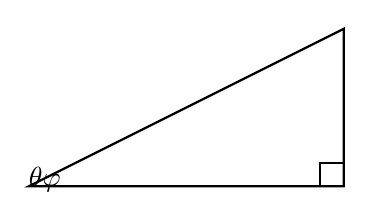
\begin{tikzpicture}[thick]
\coordinate (O) at (0,0);
\coordinate (A) at (4,0);
\coordinate (B) at (4,2);
\draw (O)--(A)--(B)--cycle;
%% The Right Angle
\coordinate (C) at (3.7,0);
\coordinate (D) at (3.7,0.3);
\coordinate (E) at (4,0.3);
\draw (C)--(D)--(E);
%% Line segment labeling
\tkzLabelSegment[below=2pt](O,A){b}
\tkzLabelSegment[above left=2pt](O,B){c}
\tkzLabelSegment[right=2pt](A,B){a}
%% Angle Labeling
\tkzMarkAngle[size=0.9cm,opacity=.4](A,O,B)
\tkzLabelAngle[pos = 0.7](A,O,B){$\theta$}
%% Angle Labeling
\tkzMarkAngle[size=0.65cm, opacity=.4](O,B,A)
\tkzLabelAngle[pos = 0.45](O,B,A){$\varphi$}
\end{tikzpicture}
\end{image}
     
    \begin{multipleChoice}
        \choice[correct]{Yes, I could find $\tan(\theta)$.}
        \choice[correct]{Yes, but I would need to review some resources first.}
        \choice[correct]{No, I would need to learn/relearn how to do this.}
        \choice[correct]{I don't know.}
        \choice[correct]{I don't want to answer this question right now.}
    
    \end{multipleChoice}

\end{question}

\begin{explanation}

    If $a, b,$ and $c$ represent the side lengths of the triangle below, could you find $a$ when $b = 3$ and $c = 8$?
    

    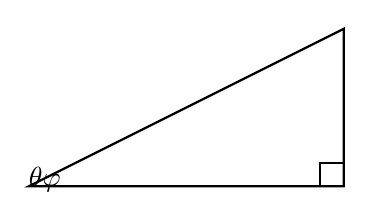
\begin{tikzpicture}[thick]
\coordinate (O) at (0,0);
\coordinate (A) at (4,0);
\coordinate (B) at (4,2);
\draw (O)--(A)--(B)--cycle;
%% The Right Angle
\coordinate (C) at (3.7,0);
\coordinate (D) at (3.7,0.3);
\coordinate (E) at (4,0.3);
\draw (C)--(D)--(E);
%% Line segment labeling
\tkzLabelSegment[below=2pt](O,A){b}
\tkzLabelSegment[above left=2pt](O,B){c}
\tkzLabelSegment[right=2pt](A,B){a}
%% Angle Labeling
\tkzMarkAngle[size=0.9cm,opacity=.4](A,O,B)
\tkzLabelAngle[pos = 0.7](A,O,B){$\theta$}
%% Angle Labeling
\tkzMarkAngle[size=0.65cm, opacity=.4](O,B,A)
\tkzLabelAngle[pos = 0.45](O,B,A){$\varphi$}
\end{tikzpicture}
     
    \begin{multipleChoice}
        \choice[correct]{Yes, I could find $a$.}
        \choice[correct]{Yes, but I would need to review some resources first.}
        \choice[correct]{No, I would need to learn/relearn how to find $a$.}
        \choice[correct]{I don't know.}
        \choice[correct]{I don't want to answer this question right now.}
    
    \end{multipleChoice}

\end{explanation}


%Content Questions

\begin{problem} 

\begin{problem}
    What is the value of $\sin(0)$?
    
    \begin{hint}
    HINT!
    \end{hint}

  \begin{multipleChoice}
      \choice[correct]{$0$}
      \choice{$1$}
      \choice{$\cfrac{\pi}{2}$}
      \choice{$\cfrac{\pi}{4}$}
      \choice{$\pi$}
      \choice{$2\pi$}
      \choice{$\cfrac{\sqrt{2}}{2}$}
      \choice{$\cfrac{1}{2}$}
      \choice{$\cfrac{\sqrt{3}}{2}$}
      
      \begin{feedback}[attempt]
          Feedback.
      \end{feedback}
      
  \end{multipleChoice}
  
\end{problem}

\begin{question}
  
  If you didn't, why didn't you answer the above question?
  
  \begin{multipleChoice}
      \choice[correct]{I don't know the answer to this question yet.}
      \choice[correct]{I don't want to answer this question right now.}
      \choice[correct]{I have already answered this question correctly.}  
      
      \begin{feedback}[attempt]
      Feedback.
      \end{feedback}
  \end{multipleChoice}
  
\end{question}

\end{problem}

\begin{problem} 

\begin{problem}
    Evaluate $\cos(x)$ at $x = \cfrac{\pi}{6}$.
    
    \begin{hint}
    HINT!
    \end{hint}

  \begin{multipleChoice}
      \choice{$0$}
      \choice{$1$}
      \choice{$\cfrac{\pi}{2}$}
      \choice{$\cfrac{\pi}{4}$}
      \choice{$\pi$}
      \choice{$2\pi$}
      \choice{$\cfrac{\sqrt{2}}{2}$}
      \choice{$\cfrac{1}{2}$}
      \choice[correct]{$\cfrac{\sqrt{3}}{2}$}
      
      \begin{feedback}[attempt]
          Feedback.
      \end{feedback}
      
  \end{multipleChoice}
  
\end{problem}

\begin{question}
  
    If you didn't, why didn't you answer the above question?
  
  \begin{multipleChoice}
      \choice[correct]{I don't know the answer to this question yet.}
      \choice[correct]{I don't want to answer this question right now.}
      \choice[correct]{I have already answered this question correctly.}  
      
      \begin{feedback}[attempt]
      Feedback.
      \end{feedback}
  \end{multipleChoice}
  
\end{question}

\end{problem}

\begin{problem} 

\begin{problem}
    What is the trigonometric function whose graph is below?
    
    \begin{center} \includegraphics[scale=0.3]{TrigGraph.png} \end{center}
    
    \begin{hint}
    HINT!
    \end{hint}

  \begin{multipleChoice}
      \choice[correct]{$\sin(x)$}
      \choice{$\cos(x)$}
      \choice{$\tan(x)$}
      \choice{$\sec(x)$}
      \choice{$\csc(x)$}
      \choice{$\cot(x)$}
      
      \begin{feedback}[attempt]
          Feedback.
      \end{feedback}
      
  \end{multipleChoice}
  
\end{problem}

\begin{question}
  
    If you didn't, why didn't you answer the above question?
  
  \begin{multipleChoice}
      \choice[correct]{I don't know the answer to this question yet.}
      \choice[correct]{I don't want to answer this question right now.}
      \choice[correct]{I have already answered this question correctly.}  
      
      \begin{feedback}[attempt]
      Feedback.
      \end{feedback}
  \end{multipleChoice}
  
\end{question}

\end{problem}

\begin{problem} 

\begin{problem}
    
    If $a, b,$ and $c$ represent the side lengths of the triangle below, find $\tan(\theta)$ when $a = 3$, $b = 4$, and $c = 8$.  (Choose all correct answers)
    
    \begin{center}
    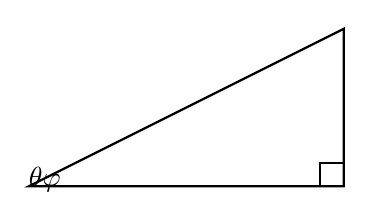
\begin{tikzpicture}[thick]
\coordinate (O) at (0,0);
\coordinate (A) at (4,0);
\coordinate (B) at (4,2);
\draw (O)--(A)--(B)--cycle;
%% The Right Angle
\coordinate (C) at (3.7,0);
\coordinate (D) at (3.7,0.3);
\coordinate (E) at (4,0.3);
\draw (C)--(D)--(E);
%% Line segment labeling
\tkzLabelSegment[below=2pt](O,A){b}
\tkzLabelSegment[above left=2pt](O,B){c}
\tkzLabelSegment[right=2pt](A,B){a}
%% Angle Labeling
\tkzMarkAngle[size=0.9cm,opacity=.4](A,O,B)
\tkzLabelAngle[pos = 0.7](A,O,B){$\theta$}
%% Angle Labeling
\tkzMarkAngle[size=0.65cm, opacity=.4](O,B,A)
\tkzLabelAngle[pos = 0.45](O,B,A){$\varphi$}
\end{tikzpicture}
    \end{center}
    
    \begin{hint}
    HINT!
    \end{hint}

  \begin{selectAll}
      \choice{$\cfrac{4}{3}$}
      \choice[correct]{$\cfrac{3}{4}$}
      \choice{$\cfrac{5}{3}$}
      \choice{$\cfrac{3}{5}$}
      \choice{$\cfrac{4}{5}$}
      \choice{$\cfrac{5}{4}$}
      \choice{$\tan^{-1}\left(\frac{5}{4}\right)$}
      \choice{You cannot answer this question without a calculator.}
      \choice{You cannot answer this question without knowing $\theta$.}
      
      \begin{feedback}[attempt]
          Feedback.
      \end{feedback}
      
  \end{selectAll}
  
\end{problem}

\begin{question}
  
    If you didn't, why didn't you answer the above question?
  
  \begin{multipleChoice}
      \choice[correct]{I don't know the answer to this question yet.}
      \choice[correct]{I don't want to answer this question right now.}
      \choice[correct]{I have already answered this question correctly.}  
      
      \begin{feedback}[attempt]
      Feedback.
      \end{feedback}
  \end{multipleChoice}
  
\end{question}

\end{problem}

\begin{problem} 

\begin{problem}
    
    If $a, b,$ and $c$ represent the side lengths of the triangle below, find $a$ when $b = 3$ and $c = 8$.
    
    \begin{center}
    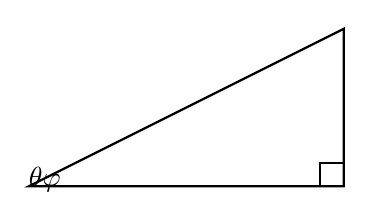
\begin{tikzpicture}[thick]
\coordinate (O) at (0,0);
\coordinate (A) at (4,0);
\coordinate (B) at (4,2);
\draw (O)--(A)--(B)--cycle;
%% The Right Angle
\coordinate (C) at (3.7,0);
\coordinate (D) at (3.7,0.3);
\coordinate (E) at (4,0.3);
\draw (C)--(D)--(E);
%% Line segment labeling
\tkzLabelSegment[below=2pt](O,A){b}
\tkzLabelSegment[above left=2pt](O,B){c}
\tkzLabelSegment[right=2pt](A,B){a}
%% Angle Labeling
\tkzMarkAngle[size=0.9cm,opacity=.4](A,O,B)
\tkzLabelAngle[pos = 0.7](A,O,B){$\theta$}
%% Angle Labeling
\tkzMarkAngle[size=0.65cm, opacity=.4](O,B,A)
\tkzLabelAngle[pos = 0.45](O,B,A){$\varphi$}
\end{tikzpicture}
    \end{center}
    
    \begin{hint}
    HINT!
    \end{hint}

  \begin{multipleChoice}
      \choice{$73$}
      \choice{$\sqrt{73}$}
      \choice[correct]{$\sqrt{55}$}
      \choice{$55$}
      \choice{$5$}
      \choice{$\sqrt{5}$}
      \choice{$\cfrac{8}{3}$}
      \choice{$\cos^{-1}\left(\frac{8}{3}\right)$}
      
      \begin{feedback}[attempt]
          Feedback.
      \end{feedback}
      
  \end{multipleChoice}
  
\end{problem}

\begin{question}
  
    If you didn't, why didn't you answer the above question?
  
  \begin{multipleChoice}
      \choice[correct]{I don't know the answer to this question yet.}
      \choice[correct]{I don't want to answer this question right now.}
      \choice[correct]{I have already answered this question correctly.}  
      
      \begin{feedback}[attempt]
      Feedback.
      \end{feedback}
  \end{multipleChoice}
  
\end{question}

\end{problem}

%Self-Control Questions

\begin{center} \textbf{Strategy Reflection}\end{center}

\begin{question}

Below are statements about strategies that you may or may not have used while completing the above questions.  Mark true or false to indicate whether each statement describes how you took this pre-quiz. 

\begin{question}

    A. I answered the questions in order, assuming that the easier ones would come first.

    \begin{multipleChoice}
        \choice[correct]{True}
        \choice[correct]{False}
    \end{multipleChoice}
    
\end{question}
\begin{question}
    
    B. I answered the questions that I knew how to do first.

    \begin{multipleChoice}
        \choice[correct]{True}
        \choice[correct]{False}
    \end{multipleChoice}
    
\end{question}

\begin{question}
    
    C. I read through all of the questions first before answering any.

    \begin{multipleChoice}
        \choice[correct]{True}
        \choice[correct]{False}
    \end{multipleChoice}
    
\end{question}
\begin{question}
    
    D. After reading a question, I worked backwards and used process of elimination to narrow down my options by checking if the answers were correct.

    \begin{multipleChoice}
        \choice[correct]{True}
        \choice[correct]{False}
    \end{multipleChoice}
    
\end{question}

\begin{question}
    
    E. When working on a problem, I solved the question by myself without the answers first, and then I tried to find the appropriate answer.

    \begin{multipleChoice}
        \choice[correct]{True}
        \choice[correct]{False}
    \end{multipleChoice}
    
\end{question}

\begin{question}
    
    F. I used the unit circle to determine values of the functions.

    \begin{multipleChoice}
        \choice[correct]{True}
        \choice[correct]{False}
    \end{multipleChoice}
    
\end{question}

\begin{question}
    
    G. I solved the questions the way I knew how and then determined if any of the other answers were equivalent.

    \begin{multipleChoice}
        \choice[correct]{True}
        \choice[correct]{False}
    \end{multipleChoice}
    
\end{question}

\begin{question}
    
    H. I tested values from the answers to determine if they were correct or not.

    \begin{multipleChoice}
        \choice[correct]{True}
        \choice[correct]{False}
    \end{multipleChoice}
    
\end{question}

\begin{question}    
    
    I. I used online resources to find the solutions.

    \begin{multipleChoice}
        \choice[correct]{True}
        \choice[correct]{False}
    \end{multipleChoice}
    
\end{question}
\begin{question}    
    
    J. I used online resources to remind me how to answer the questions, but then solved them myself.

    \begin{multipleChoice}
        \choice[correct]{True}
        \choice[correct]{False}
    \end{multipleChoice}
    
\end{question}
\begin{question}    
    
    K. I used strategies when completing this pre-quiz, but I don't remember the names of the strategies.

    \begin{multipleChoice}
        \choice[correct]{True}
        \choice[correct]{False}
    \end{multipleChoice}
    
\end{question}
\begin{question}    
    
    L. I used other strategies that are not listed here.

    \begin{multipleChoice}
        \choice[correct]{True}
        \choice[correct]{False}
    \end{multipleChoice}
    
\end{question}
\begin{question}    
    
    M. I did not use any strategies when completing this pre-quiz.

    \begin{multipleChoice}
        \choice[correct]{True}
        \choice[correct]{False}
    \end{multipleChoice}

\end{question}
\end{question}


\begin{question}
    Please list any additional strategies that you used when taking this pre-quiz. If you didn't use any additional strategies, just type `NA.`
   \begin{freeResponse}
   \end{freeResponse}
\end{question}



%\input{../leveledQuestions.tex}


\end{document}
